% Generated by build/sync_qft_soln.py from committed sources only.
% Source repository: https://github.com/Luca-Yucheng-Jin/QFT-soln
% Source commit: 07d7fe95fd5cf5b26d38a16ee535a04a925277b2
\section{Generating Functionals for $\phi^4$ (PSI QFT II, Homework 1)}

\noindent\textit{Question prompts paraphrased from the official
\href{https://psi-online.perimeterinstitute.ca/courses/take/quantum-field-theory-ii-student/pdfs/20776374-module-3-homework}{Perimeter PSI Online sheet};
the equations and notation follow the source.}

\subsection{Computing Correlation Functions Using Generating Functionals}

Work in Euclidean signature with the interacting scalar-field action
\begin{equation}
    S[\phi]=S_0[\phi]+\int d^4x\,V(\phi),
    \qquad
    V(\phi)=\frac{g}{4!}\phi^4,
\end{equation}
where $S_0[\phi]$ is the free Euclidean action.

\begin{enumerate}[label=\alph*)]
    \item Introduce a source $J(x)$ and consider the free generating functional
    \begin{equation}
        \mathcal Z_0[J]
        =\int\mathcal D\phi\,
        \exp\!\left[
            -\frac{1}{\hbar}
            \left(
                S_0[\phi]-\int d^4x\,J(x)\phi(x)
            \right)
        \right].
    \end{equation}
    Evaluate this Gaussian functional integral. As a hint, first shift the integration
    variable by a function determined by $J$.
    \begin{solution}
        In the Euclidean picture, we have
        \begin{equation}
            S_0[\phi] = -\frac{1}{2}\phi (\partial^2 - m^2)\phi.
        \end{equation}
        To evaluate the integral, we make the shift of the integration variable,
        \begin{equation}
            \bar \phi(x) = \phi(x) + \int d^dy \Delta(x-y)J(y) \equiv \phi_x + \Delta_{xy}J_y,
        \end{equation}
        where we have used the generalised summation convention and $(\partial^2 - m^2)\Delta(x-y) = \delta^d(x-y)$. Since $\mathcal{D}\phi = \mathcal{D}\bar \phi$, we have
        \begin{equation}
        \begin{aligned}
            Z_0[J] &= \int \mathcal{D}\bar \phi\exp\left[-\frac{1}{\hbar}\left(-\frac{1}{2}\bar \phi_x(\partial^2-m^2)_{xy}\bar \phi_y + \frac{1}{2}J_x\Delta_{xy}J_y\right)\right]  \\
            &=\exp\left[-\frac{1}{\hbar}\int d^dx\int d^dy \frac{1}{2}J(x)\Delta(x-y)J(y)\right]Z_0[0].
        \end{aligned}
        \end{equation}
    \end{solution}

    \item For an arbitrary polynomial interaction $V(\phi)$, establish the identity
    \begin{align}
        &\exp\!\left[
            -\frac{1}{\hbar}\int d^4x\,V(\phi)
            +\frac{1}{\hbar}\int d^4x\,J(x)\phi(x)
        \right]
        \notag\\
        &\qquad=
        \exp\!\left[
            -\frac{1}{\hbar}\int d^4x\,
            V\!\left(\hbar\frac{\delta}{\delta J(x)}\right)
        \right]
        \exp\!\left[
            \frac{1}{\hbar}\int d^4x\,J(x)\phi(x)
        \right].
    \end{align}
    \begin{solution}
        \begin{equation}
            \begin{aligned}
                &\exp\!\left[
            -\frac{1}{\hbar}\int d^4x\,V(\phi)
            +\frac{1}{\hbar}\int d^4x\,J(x)\phi(x)
        \right]\\ &= \sum_{n=0}^\infty\frac{1}{n!}\left(-\frac{1}{\hbar}\right)^n\left(\int d^dxV(\phi)\right)^n\exp\left(\frac{1}{\hbar}\int d^dx J(x) \phi(x)\right)\\
        &=\sum_{n=0}^\infty\frac{1}{n!}\left(-\frac{1}{\hbar}\right)^n\left(\int d^dx V\left(\hbar \frac{\delta}{\delta J(x)}\right)\right)^n\exp\left(\frac{1}{\hbar}\int d^dx J(x) \phi(x)\right)\\
        &=\exp\!\left[
            -\frac{1}{\hbar}\int d^4x\,
            V\!\left(\hbar\frac{\delta}{\delta J(x)}\right)
        \right]
        \exp\!\left[
            \frac{1}{\hbar}\int d^4x\,J(x)\phi(x)
        \right].
            \end{aligned}
        \end{equation}
    \end{solution}

    \item For the interacting theory, define
    \begin{equation}
        \mathcal Z[J]
        =\int\mathcal D\phi\,
        \exp\!\left[
            -\frac{1}{\hbar}
            \left(
                S[\phi]-\int d^4x\,J(x)\phi(x)
            \right)
        \right].
    \end{equation}
    Use the preceding result to express $\mathcal Z[J]$ formally as a functional
    differential operator acting on $\mathcal Z_0[J]$.
    \begin{solution}
        From b), we have
        \begin{equation}
            Z[J] = \int \mathcal{D}\phi\exp\!\left[
            -\frac{1}{\hbar}\int d^4x\,
            V\!\left(\hbar\frac{\delta}{\delta J(x)}\right)
        \right]\exp\!\left[
            -\frac{1}{\hbar}
            \left(
                S_0[\phi]-\int d^4x\,J(x)\phi(x)
            \right)
        \right].
        \end{equation}
        Then, using the same field redefinition in a), we find
        \begin{equation}
            Z[J] = \exp\!\left[
            -\frac{1}{\hbar}\int d^4x\,
            V\!\left(\hbar\frac{\delta}{\delta J(x)}\right)
        \right]\exp\left[-\frac{1}{\hbar}\int d^dx\int d^dy \frac{1}{2}J(x)\Delta(x-y)J(y)\right]Z_0[0],
        \end{equation}
        or equivalently,
        \begin{equation}
            Z[J] = \exp\!\left[
            -\frac{1}{\hbar}\int d^4x\,
            V\!\left(\hbar\frac{\delta}{\delta J(x)}\right)
        \right]Z_0[J].
        \end{equation}
    \end{solution}

    \item The two-point Green function may be obtained from
    \begin{equation}
        G(x_1,x_2)
        =\langle\phi(x_1)\phi(x_2)\rangle
        =\left.
        \frac{\hbar^2}{\mathcal Z[0]}
        \frac{\delta^2\mathcal Z[J]}
             {\delta J(x_1)\delta J(x_2)}
        \right|_{J=0}.
    \end{equation}
    Compute its perturbative expansion through order $g^2$ in $\phi^4$ theory.
    At each order, list every contribution without evaluating the position-space
    integrals, draw its Feynman diagram, and give the correct symmetry factor.
    \begin{solution}
        Using the results from above, we have
        \begin{equation}
            G(x_1,x_2) = \hbar^2\frac{\delta^2}{\delta_1 \delta_2}\exp\!\left[
            -\frac{1}{\hbar}\int d^4x\,
            V\!\left(\hbar\frac{\delta}{\delta_x}\right)
        \right]\exp\left[-\frac{1}{\hbar} \frac{1}{2}J_x\Delta_{xy}J_y\right]\bigg|_{J=0}\frac{Z_0[0]}{Z[0]},
        \end{equation}
        where $Z[0]$ can be written as
        \begin{equation}
            Z[0] = \exp\!\left[
            -\frac{1}{\hbar}\int d^4x\,
            V\!\left(\hbar\frac{\delta}{\delta_x}\right)
        \right]\exp\left[-\frac{1}{\hbar} \frac{1}{2}J_x\Delta_{xy}J_y\right]\bigg|_{J=0}Z_0[0].
        \end{equation}
        Expanding the first exponential to order $g^2$, we have
        \begin{equation}
            \begin{aligned}
                \exp\!\left[-\frac{1}{\hbar}\int d^4x\,
                    V\!\left(\hbar\frac{\delta}{\delta_x}\right)\right]
                ={}&1-\frac{1}{\hbar}\frac{g}{4!}\int d^dx\,
                    \left(\hbar \frac{\delta}{\delta_x}\right)^4\\
                &+\frac{1}{2\hbar^2}\left(\frac{g}{4!}\right)^2
                    \int d^dx\,
                    \left(\hbar \frac{\delta}{\delta_x}\right)^4
                    \int d^dy\,
                    \left(\hbar \frac{\delta}{\delta_y}\right)^4
                    +\cdots.
            \end{aligned}
        \end{equation}
        At order $g^0$, we simply have $Z[0]=Z_0[0]$, and hence
        \begin{equation}
            G_{12} = -\hbar\Delta_{12} + \cdots.
        \end{equation}
        At order $g^1$, we need to evaluate
        \begin{equation}
            \begin{aligned}
                &\left(\hbar \frac{\delta}{\delta_x}\right)^4\exp\left[-\frac{1}{\hbar} \frac{1}{2}J_x\Delta_{xy}J_y\right]\\
                &=\left(\hbar \frac{\delta}{\delta_x}\right)^3\left(-\Delta_{xy}J_y\exp\left[-\frac{1}{\hbar} \frac{1}{2}J_x\Delta_{xy}J_y\right]\right)\\
                &=\left(\hbar \frac{\delta}{\delta_x}\right)^2\left((-\hbar\Delta_{xx}+\Delta_{xy}\Delta_{xz}J_yJ_z)\exp\left[-\frac{1}{\hbar} \frac{1}{2}J_x\Delta_{xy}J_y\right]\right)\\
                &=\left(\hbar \frac{\delta}{\delta_x}\right)\left((3\hbar\Delta_{xx}\Delta_{xy}J_y-\Delta_{xy}\Delta_{xz}\Delta_{xw}J_yJ_zJ_w)\exp\left[-\frac{1}{\hbar} \frac{1}{2}J_x\Delta_{xy}J_y\right]\right)\\
                &=\left((3\hbar^2\Delta_{xx}\Delta_{xx}-6\hbar\Delta_{xy}\Delta_{xz}\Delta_{xx}J_yJ_z + \Delta_{xy}\Delta_{xz}\Delta_{xw}\Delta_{xu}J_yJ_zJ_wJ_u)\exp\left[-\frac{1}{\hbar} \frac{1}{2}J_x\Delta_{xy}J_y\right]\right).
            \end{aligned}
        \end{equation}
        From this, we can read out
        \begin{equation}
            Z[0] = Z_0[0]\left(1-\frac{g}{8}\hbar\int d^dx\Delta_{xx}^2+\cdots\right).
        \end{equation}
        Diagrammatically, the order-$g$ vacuum contribution is
        \begin{equation}
            \frac{Z[0]}{Z_0[0]}
            =1+
            \vcenter{\hbox{%
            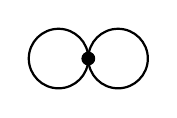
\begin{tikzpicture}[
                baseline=(current bounding box.center),
                scale=1.35,
                transform shape,
                psihwOneScalar/.style={draw=black,line width=0.8pt},
                psihwOneVertex/.style={circle,fill=black,draw=black,
                                       minimum size=3.4pt,inner sep=0pt}]
                \coordinate (v) at (0,0);
                \draw[psihwOneScalar] (v) ++(-0.28,0) circle (0.28);
                \draw[psihwOneScalar] (v) ++( 0.28,0) circle (0.28);
                \node[psihwOneVertex] at (v) {};
            \end{tikzpicture}}}
            +\cdots,
            \qquad S=8.
        \end{equation}
        Hence
        \begin{equation}
            \begin{aligned}
                G_{12}
                &=\left[-\hbar\Delta_{12}
                +\frac{g}{8}\hbar^2\Delta_{12}\int d^dx\,\Delta_{xx}^2
                +\frac{g}{2}\hbar^2\int d^dx\,
                    \Delta_{xx}\Delta_{1x}\Delta_{2x}
                +\mathcal O(g^2)\right]\\
                &\quad\times
                \left[1+\frac{g}{8}\hbar\int d^dy\,\Delta_{yy}^2
                +\mathcal O(g^2)\right]\\
                &=-\hbar\Delta_{12}
                +\frac{g}{2}\hbar^2\int d^dx\,
                    \Delta_{xx}\Delta_{1x}\Delta_{2x}
                +\mathcal O(g^2).
            \end{aligned}
        \end{equation}
        The disconnected free propagator times the vacuum bubble has cancelled.
        The surviving diagrams are
        \begin{equation}
            G_{12}
            =
            \vcenter{\hbox{%
            \begin{tikzpicture}[
                baseline=(current bounding box.center),
                scale=1.35,
                transform shape,
                psihwOneScalar/.style={draw=black,line width=0.8pt},
                every node/.style={font=\scriptsize}]
                \begin{feynman}
                    \vertex (fL) at (0,0) {$x_1$};
                    \vertex (fR) at (1.45,0) {$x_2$};
                    \diagram*{(fL) -- [psihwOneScalar] (fR)};
                \end{feynman}
            \end{tikzpicture}}}
            +
            \vcenter{\hbox{%
            \begin{tikzpicture}[
                baseline=(current bounding box.center),
                scale=1.35,
                transform shape,
                psihwOneScalar/.style={draw=black,line width=0.8pt},
                psihwOneVertex/.style={circle,fill=black,draw=black,
                                       minimum size=3.4pt,inner sep=0pt},
                every node/.style={font=\scriptsize}]
                \begin{feynman}
                    \vertex (tL) at (0,0) {$x_1$};
                    \vertex[psihwOneVertex] (tV) at (0.80,0) {};
                    \vertex (tR) at (1.60,0) {$x_2$};
                    \diagram*{
                        (tL) -- [psihwOneScalar] (tV),
                        (tV) -- [psihwOneScalar] (tR),
                    };
                    \draw[psihwOneScalar] (tV) ++(0,0.28) circle (0.28);
                \end{feynman}
            \end{tikzpicture}}}
            +\mathcal O(g^2),
            \qquad S_{g^0}=1,\quad S_{g^1}=2.
        \end{equation}
        Now, we turn to order $g^2$, where we need to evaluate
        \begin{equation}
            \begin{aligned}
                &\left(\hbar \frac{\delta}{\delta_x}\right)^4
                \left(\hbar \frac{\delta}{\delta_y}\right)^4
                \exp\left[-\frac{1}{\hbar}\frac{1}{2}
                    J_x\Delta_{xy}J_y\right]\\
                &=\left(\hbar \frac{\delta}{\delta_y}\right)^4
                \Bigg[\Big(
                    3\hbar^2\Delta_{xx}^2
                    -6\hbar\Delta_{xx}\Delta_{xv}\Delta_{xw}J_vJ_w
                    +\Delta_{xv}\Delta_{xw}\Delta_{xz}\Delta_{xu}
                        J_vJ_wJ_zJ_u
                \Big)
                \exp\left[-\frac{1}{\hbar}\frac{1}{2}
                    J_x\Delta_{xy}J_y\right]\Bigg]\\
                &=\Bigg\{
                -\hbar^3\Big[
                    18\Delta_{xx}
                    \left(\Delta_{xx}\Delta_{yy}+4\Delta_{xy}^2\right)
                    \Delta_{yr}\Delta_{ys}J_rJ_s\\
                &\qquad\qquad
                    +48\Delta_{xy}
                    \left(3\Delta_{xx}\Delta_{yy}+2\Delta_{xy}^2\right)
                    \Delta_{xv}\Delta_{yr}J_vJ_r\\
                &\qquad\qquad
                    +18\Delta_{yy}
                    \left(\Delta_{xx}\Delta_{yy}+4\Delta_{xy}^2\right)
                    \Delta_{xv}\Delta_{xw}J_vJ_w
                \Big]\\
                &\qquad
                +\hbar^4\Big(
                    9\Delta_{xx}^2\Delta_{yy}^2
                    +72\Delta_{xx}\Delta_{yy}\Delta_{xy}^2
                    +24\Delta_{xy}^4
                \Big)\Bigg\}
                \exp\left[-\frac{1}{\hbar}\frac{1}{2}
                    J_x\Delta_{xy}J_y\right]\\
                &\qquad
                +\text{terms containing more than two currents}.
            \end{aligned}
        \end{equation}
        We have discarded terms with more than two currents because they vanish
        after the two external derivatives are taken and $J$ is set to zero.
        From this, we find
        \begin{equation}
            \begin{aligned}
                Z[0]=Z_0[0]\Bigg[1
                &-\frac{g}{8}\hbar\int d^dx\,\Delta_{xx}^2\\
                &+g^2\hbar^2\int d^dx\,d^dy\left(
                    \frac{1}{128}\Delta_{xx}^2\Delta_{yy}^2
                    +\frac{1}{16}\Delta_{xx}\Delta_{yy}\Delta_{xy}^2
                    +\frac{1}{48}\Delta_{xy}^4
                \right)+\mathcal O(g^3)\Bigg].
            \end{aligned}
        \end{equation}
        The three order-$g^2$ vacuum diagrams are
        \begin{equation}
            \vcenter{\hbox{%
            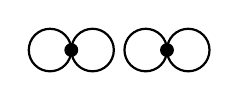
\begin{tikzpicture}[
                baseline=(current bounding box.center),
                scale=1.35,
                transform shape,
                psihwOneScalar/.style={draw=black,line width=0.8pt},
                psihwOneVertex/.style={circle,fill=black,draw=black,
                                       minimum size=3.4pt,inner sep=0pt}]
                \coordinate (dL) at (0.35,0);
                \coordinate (dR) at (1.25,0);
                \foreach \v in {dL,dR}{
                    \draw[psihwOneScalar] (\v) ++(-0.20,0) circle (0.20);
                    \draw[psihwOneScalar] (\v) ++( 0.20,0) circle (0.20);
                    \node[psihwOneVertex] at (\v) {};
                }
            \end{tikzpicture}}}_{S=128}
            \quad+\quad
            \vcenter{\hbox{%
            \begin{tikzpicture}[
                baseline=(current bounding box.center),
                scale=1.35,
                transform shape,
                psihwOneScalar/.style={draw=black,line width=0.8pt},
                psihwOneVertex/.style={circle,fill=black,draw=black,
                                       minimum size=3.4pt,inner sep=0pt}]
                \begin{feynman}
                    \vertex[psihwOneVertex] (mL) at (0,0) {};
                    \vertex[psihwOneVertex] (mR) at (0.95,0) {};
                    \diagram*{
                        (mL) -- [psihwOneScalar,bend left=48] (mR),
                        (mL) -- [psihwOneScalar,bend right=48] (mR),
                    };
                    \draw[psihwOneScalar] (mL) ++(-0.25,0) circle (0.25);
                    \draw[psihwOneScalar] (mR) ++( 0.25,0) circle (0.25);
                \end{feynman}
            \end{tikzpicture}}}_{S=16}
            \quad+\quad
            \vcenter{\hbox{%
            \begin{tikzpicture}[
                baseline=(current bounding box.center),
                scale=1.35,
                transform shape,
                psihwOneScalar/.style={draw=black,line width=0.8pt},
                psihwOneVertex/.style={circle,fill=black,draw=black,
                                       minimum size=3.4pt,inner sep=0pt}]
                \begin{feynman}
                    \vertex[psihwOneVertex] (bL) at (0,0) {};
                    \vertex[psihwOneVertex] (bR) at (1.10,0) {};
                    \diagram*{
                        (bL) -- [psihwOneScalar,bend left=25] (bR),
                        (bL) -- [psihwOneScalar,bend left=65] (bR),
                        (bL) -- [psihwOneScalar,bend right=25] (bR),
                        (bL) -- [psihwOneScalar,bend right=65] (bR),
                    };
                \end{feynman}
            \end{tikzpicture}}}_{S=48}.
        \end{equation}
        As at order $g$, all vacuum-disconnected terms cancel against the
        normalization by $Z[0]$. The connected result is therefore
        \begin{equation}
            \begin{aligned}
                G_{12}={}&-\hbar\Delta_{12}
                +\frac{g}{2}\hbar^2\int d^dx\,
                    \Delta_{1x}\Delta_{xx}\Delta_{x2}\\
                &-g^2\hbar^3\int d^dx\,d^dy\Bigg(
                    \frac{1}{4}\Delta_{1x}\Delta_{2x}
                        \Delta_{xy}^2\Delta_{yy}
                    +\frac{1}{4}\Delta_{1x}\Delta_{xx}
                        \Delta_{xy}\Delta_{yy}\Delta_{y2}\\
                &\hspace{45mm}
                    +\frac{1}{6}\Delta_{1x}\Delta_{xy}^3\Delta_{y2}
                \Bigg)+\mathcal O(g^3).
            \end{aligned}
        \end{equation}
        The order-$g^2$ terms are, in the same order as in the preceding equation,
        \begin{equation}
            \vcenter{\hbox{%
            \begin{tikzpicture}[
                baseline=(current bounding box.center),
                scale=1.35,
                transform shape,
                psihwOneScalar/.style={draw=black,line width=0.8pt},
                psihwOneVertex/.style={circle,fill=black,draw=black,
                                       minimum size=3.4pt,inner sep=0pt},
                every node/.style={font=\scriptsize}]
                \begin{feynman}
                    \vertex (q1) at (0,0.43) {$x_1$};
                    \vertex (q2) at (0,-0.43) {$x_2$};
                    \vertex[psihwOneVertex] (qx) at (0.62,0) {};
                    \vertex[psihwOneVertex] (qy) at (1.52,0) {};
                    \diagram*{
                        (q1) -- [psihwOneScalar] (qx),
                        (q2) -- [psihwOneScalar] (qx),
                        (qx) -- [psihwOneScalar,bend left=52] (qy),
                        (qx) -- [psihwOneScalar,bend right=52] (qy),
                    };
                    \draw[psihwOneScalar] (qy) ++(0.25,0) circle (0.25);
                \end{feynman}
            \end{tikzpicture}}}_{S=4}
            \quad+\quad
            \vcenter{\hbox{%
            \begin{tikzpicture}[
                baseline=(current bounding box.center),
                scale=1.35,
                transform shape,
                psihwOneScalar/.style={draw=black,line width=0.8pt},
                psihwOneVertex/.style={circle,fill=black,draw=black,
                                       minimum size=3.4pt,inner sep=0pt},
                every node/.style={font=\scriptsize}]
                \begin{feynman}
                    \vertex (c1) at (0,0) {$x_1$};
                    \vertex[psihwOneVertex] (cx) at (0.55,0) {};
                    \vertex[psihwOneVertex] (cy) at (1.45,0) {};
                    \vertex (c2) at (2.00,0) {$x_2$};
                    \diagram*{
                        (c1) -- [psihwOneScalar] (cx),
                        (cx) -- [psihwOneScalar] (cy),
                        (cy) -- [psihwOneScalar] (c2),
                    };
                    \draw[psihwOneScalar] (cx) ++(0,0.25) circle (0.25);
                    \draw[psihwOneScalar] (cy) ++(0,0.25) circle (0.25);
                \end{feynman}
            \end{tikzpicture}}}_{S=4}
            \quad+\quad
            \vcenter{\hbox{%
            \begin{tikzpicture}[
                baseline=(current bounding box.center),
                scale=1.35,
                transform shape,
                psihwOneScalar/.style={draw=black,line width=0.8pt},
                psihwOneVertex/.style={circle,fill=black,draw=black,
                                       minimum size=3.4pt,inner sep=0pt},
                every node/.style={font=\scriptsize}]
                \begin{feynman}
                    \vertex (s1) at (0,0) {$x_1$};
                    \vertex[psihwOneVertex] (sx) at (0.55,0) {};
                    \vertex[psihwOneVertex] (sy) at (1.55,0) {};
                    \vertex (s2) at (2.10,0) {$x_2$};
                    \diagram*{
                        (s1) -- [psihwOneScalar] (sx),
                        (sx) -- [psihwOneScalar] (sy),
                        (sx) -- [psihwOneScalar,bend left=55] (sy),
                        (sx) -- [psihwOneScalar,bend right=55] (sy),
                        (sy) -- [psihwOneScalar] (s2),
                    };
                \end{feynman}
            \end{tikzpicture}}}_{S=6}.
        \end{equation}
    \end{solution}

    \item Mark the one-particle-irreducible subgraphs in the diagrams obtained in the
    previous part.

    \begin{solution}
        \begin{center}
            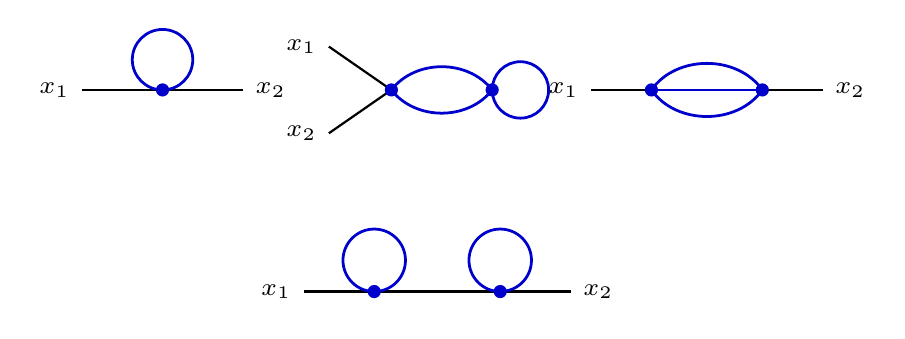
\begin{tikzpicture}[
                scale=1.28,
                transform shape,
                psihwOneScalar/.style={draw=black,line width=0.8pt},
                psihwOnePI/.style={draw=blue!80!black,line width=1pt},
                psihwOneVertex/.style={circle,fill=black,draw=black,
                                       minimum size=3.4pt,inner sep=0pt},
                psihwOnePIVertex/.style={circle,fill=blue!80!black,draw=blue!80!black,
                                         minimum size=3.4pt,inner sep=0pt},
                every node/.style={font=\scriptsize}]
                % Order-g tadpole: the whole amputated core is 1PI.
                \coordinate (tL) at (0,1.45);
                \coordinate (tV) at (0.80,1.45);
                \coordinate (tR) at (1.60,1.45);
                \draw[psihwOneScalar] (tL)--(tV) (tV)--(tR);
                \draw[psihwOnePI] (tV) ++(0,0.30) circle (0.30);
                \node[psihwOnePIVertex] at (tV) {};
                \node[left] at (tL) {$x_1$};
                \node[right] at (tR) {$x_2$};


                % Nested order-g^2 diagram: the complete core is 1PI.
                \coordinate (q1) at (2.45,1.88);
                \coordinate (q2) at (2.45,1.02);
                \coordinate (qx) at (3.07,1.45);
                \coordinate (qy) at (4.07,1.45);
                \draw[psihwOneScalar] (q1)--(qx) (q2)--(qx);
                \draw[psihwOnePI] (qx) to[bend left=52] (qy);
                \draw[psihwOnePI] (qx) to[bend right=52] (qy);
                \draw[psihwOnePI] (qy) ++(0.28,0) circle (0.28);
                \node[psihwOnePIVertex] at (qx) {};
                \node[psihwOnePIVertex] at (qy) {};
                \node[left] at (q1) {$x_1$};
                \node[left] at (q2) {$x_2$};


                % Sunset: the complete three-line core is 1PI.
                \coordinate (s1) at (5.05,1.45);
                \coordinate (sx) at (5.65,1.45);
                \coordinate (sy) at (6.75,1.45);
                \coordinate (s2) at (7.35,1.45);
                \draw[psihwOneScalar] (s1)--(sx) (sy)--(s2);
                \draw[psihwOnePI] (sx)--(sy);
                \draw[psihwOnePI] (sx) to[bend left=55] (sy);
                \draw[psihwOnePI] (sx) to[bend right=55] (sy);
                \node[psihwOnePIVertex] at (sx) {};
                \node[psihwOnePIVertex] at (sy) {};
                \node[left] at (s1) {$x_1$};
                \node[right] at (s2) {$x_2$};


                % Serial double tadpole: two 1PI insertions joined by a bridge.
                \coordinate (c1) at (2.20,-0.55);
                \coordinate (cx) at (2.90,-0.55);
                \coordinate (cy) at (4.15,-0.55);
                \coordinate (c2) at (4.85,-0.55);
                \draw[psihwOneScalar] (c1)--(cx) (cx)--(cy) (cy)--(c2);
                \draw[psihwOnePI] (cx) ++(0,0.31) circle (0.31);
                \draw[psihwOnePI] (cy) ++(0,0.31) circle (0.31);
                \node[psihwOnePIVertex] at (cx) {};
                \node[psihwOnePIVertex] at (cy) {};
                \node[left] at (c1) {$x_1$};
                \node[right] at (c2) {$x_2$};

            \end{tikzpicture}
        \end{center}
    \end{solution}

    \item Repeat the preceding two parts for the four-point correlation function,
    retaining all contributions through order $g^2$.

    \begin{solution}
        Using the results from d), we have
        \begin{equation}
            G_{1234}
            =\left.\hbar^4\frac{\delta^4}{\delta_1\delta_2\delta_3\delta_4}
            \exp\!\left[-\frac{1}{\hbar}\int d^4x\,
                V\!\left(\hbar\frac{\delta}{\delta_x}\right)\right]
            \exp\!\left[-\frac{1}{\hbar}\frac{1}{2}
                J_x\Delta_{xy}J_y\right]\right|_{J=0}
            \frac{Z_0[0]}{Z[0]}.
        \end{equation}
        As before, all vacuum-disconnected terms cancel against the
        normalization by $Z[0]$.  At order $g^0$, we find
        \begin{equation}
            G_{1234}^{(0)}
            =\hbar^2\left(
                \Delta_{12}\Delta_{34}
                +\Delta_{13}\Delta_{24}
                +\Delta_{14}\Delta_{23}
            \right).
        \end{equation}
        The remaining disconnected terms are already fixed by the two-point
        result.  For each of
        \begin{equation}
            (ij\vert kl)=(12\vert34),\ (13\vert24),\ (14\vert23),
        \end{equation}
        we obtain
        \begin{equation}
            \begin{aligned}
                G_{ij}G_{kl}={}&\hbar^2\Delta_{ij}\Delta_{kl}\\
                &-\frac{g}{2}\hbar^3\int d^dx\,\Big(
                    \Delta_{ij}\Delta_{kx}\Delta_{xx}\Delta_{xl}
                    +\Delta_{kl}\Delta_{ix}\Delta_{xx}\Delta_{xj}
                \Big)\\
                &+g^2\hbar^4\int d^dx\,d^dy\,\Bigg\{
                    \Delta_{ij}\Bigg(
                        \frac{1}{4}\Delta_{kx}\Delta_{lx}
                            \Delta_{xy}^2\Delta_{yy}
                        +\frac{1}{4}\Delta_{kx}\Delta_{xx}
                            \Delta_{xy}\Delta_{yy}\Delta_{yl}
                        +\frac{1}{6}\Delta_{kx}\Delta_{xy}^3\Delta_{yl}
                    \Bigg)\\
                &\hspace{31mm}
                    +\Delta_{kl}\Bigg(
                        \frac{1}{4}\Delta_{ix}\Delta_{jx}
                            \Delta_{xy}^2\Delta_{yy}
                        +\frac{1}{4}\Delta_{ix}\Delta_{xx}
                            \Delta_{xy}\Delta_{yy}\Delta_{yj}
                        +\frac{1}{6}\Delta_{ix}\Delta_{xy}^3\Delta_{yj}
                    \Bigg)\\
                &\hspace{31mm}
                    +\frac{1}{4}\Delta_{ix}\Delta_{xx}\Delta_{xj}
                        \Delta_{ky}\Delta_{yy}\Delta_{yl}
                \Bigg\}+\mathcal O(g^3).
            \end{aligned}
        \end{equation}
        The connected terms are
        \begin{equation}
            \begin{aligned}
                &G_{1234}-G_{12}G_{34}-G_{13}G_{24}-G_{14}G_{23}\\
                ={}&-g\hbar^3\int d^dx\,
                    \Delta_{1x}\Delta_{2x}\Delta_{3x}\Delta_{4x}\\
                &+\frac{g^2}{2}\hbar^4\int d^dx\,d^dy\,\Bigg\{
                    \Delta_{xx}\Delta_{xy}\Big(
                        \Delta_{1x}\Delta_{2y}\Delta_{3y}\Delta_{4y}
                        +\Delta_{2x}\Delta_{1y}\Delta_{3y}\Delta_{4y}\\
                &\hspace{48mm}
                        +\Delta_{3x}\Delta_{1y}\Delta_{2y}\Delta_{4y}
                        +\Delta_{4x}\Delta_{1y}\Delta_{2y}\Delta_{3y}
                    \Big)\\
                &\hspace{25mm}
                    +\Delta_{xy}^2\Big(
                        \Delta_{1x}\Delta_{2x}\Delta_{3y}\Delta_{4y}
                        +\Delta_{1x}\Delta_{3x}\Delta_{2y}\Delta_{4y}
                        +\Delta_{1x}\Delta_{4x}\Delta_{2y}\Delta_{3y}
                    \Big)
                \Bigg\}+\mathcal O(g^3).
            \end{aligned}
        \end{equation}
        These corresponds to the diagrams

        \begin{center}
            $\mathcal O(g^0):\quad$
            \begin{tikzpicture}[
                baseline=(current bounding box.center),
                scale=1.20,
                transform shape,
                psihwFourScalar/.style={draw=black,solid,line width=0.8pt},
                every node/.style={font=\scriptsize}]
                \begin{feynman}
                    \vertex (z1) at (0,0.32) {$x_1$};
                    \vertex (z2) at (1.55,0.32) {$x_2$};
                    \vertex (z3) at (0,-0.32) {$x_3$};
                    \vertex (z4) at (1.55,-0.32) {$x_4$};
                    \diagram*{
                        (z1) -- [psihwFourScalar] (z2),
                        (z3) -- [psihwFourScalar] (z4),
                    };
                \end{feynman}
                \node at (0.78,-0.78) {$3\times,\quad S=1$};
            \end{tikzpicture}
        \end{center}

        \begin{center}
            $\mathcal O(g^1):\quad$
            \begin{tikzpicture}[
                baseline=(current bounding box.center),
                scale=1.20,
                transform shape,
                psihwFourScalar/.style={draw=black,solid,line width=0.8pt},
                psihwFourPI/.style={draw=blue!80!black,solid,line width=1pt},
                psihwFourPIVertex/.style={circle,fill=blue!80!black,draw=blue!80!black,
                                          minimum size=3.4pt,inner sep=0pt},
                every node/.style={font=\scriptsize}]
                \begin{scope}
                    \begin{feynman}
                        \vertex (o1) at (0,0.52) {$x_1$};
                        \vertex (o2) at (0,-0.52) {$x_2$};
                        \vertex[psihwFourPIVertex] (ov) at (0.82,0) {};
                        \vertex (o3) at (1.64,0.52) {$x_3$};
                        \vertex (o4) at (1.64,-0.52) {$x_4$};
                        \diagram*{
                            (o1) -- [psihwFourScalar] (ov),
                            (o2) -- [psihwFourScalar] (ov),
                            (ov) -- [psihwFourScalar] (o3),
                            (ov) -- [psihwFourScalar] (o4),
                        };
                    \end{feynman}
                    \node at (0.82,-0.95) {$1\times,\quad S=1$};
                \end{scope}
                \node at (2.32,0) {$+$};
                \begin{scope}[xshift=3cm]
                    \begin{feynman}
                        \vertex (p1) at (0,0.43) {$x_1$};
                        \vertex (p2) at (1.75,0.43) {$x_2$};
                        \vertex (p3) at (0,-0.43) {$x_3$};
                        \vertex[psihwFourPIVertex] (pv) at (0.88,-0.43) {};
                        \vertex (p4) at (1.75,-0.43) {$x_4$};
                        \diagram*{
                            (p1) -- [psihwFourScalar] (p2),
                            (p3) -- [psihwFourScalar] (pv),
                            (pv) -- [psihwFourScalar] (p4),
                        };
                    \end{feynman}
                    \draw[psihwFourPI] (pv) ++(0,0.28) circle (0.28);
                    \node at (0.88,-1.02) {$6\times,\quad S=2$};
                \end{scope}
            \end{tikzpicture}
        \end{center}

        \begin{center}
            \begin{tikzpicture}[
                baseline=(current bounding box.center),
                scale=1.10,
                transform shape,
                psihwFourScalar/.style={draw=black,solid,line width=0.8pt},
                psihwFourPI/.style={draw=blue!80!black,solid,line width=1pt},
                psihwFourPIVertex/.style={circle,fill=blue!80!black,draw=blue!80!black,
                                          minimum size=3.4pt,inner sep=0pt},
                every node/.style={font=\scriptsize}]
                \node at (-0.88,2.20) {$\mathcal O(g^2):$};
                % Fish diagrams: three channels.
                \begin{scope}[shift={(0,2.20)}]
                    \begin{feynman}
                        \vertex (f1) at (0,0.48) {$x_1$};
                        \vertex (f2) at (0,-0.48) {$x_2$};
                        \vertex[psihwFourPIVertex] (fx) at (0.68,0) {};
                        \vertex[psihwFourPIVertex] (fy) at (1.68,0) {};
                        \vertex (f3) at (2.36,0.48) {$x_3$};
                        \vertex (f4) at (2.36,-0.48) {$x_4$};
                        \diagram*{
                            (f1) -- [psihwFourScalar] (fx),
                            (f2) -- [psihwFourScalar] (fx),
                            (fx) -- [psihwFourPI,bend left=50] (fy),
                            (fx) -- [psihwFourPI,bend right=50] (fy),
                            (fy) -- [psihwFourScalar] (f3),
                            (fy) -- [psihwFourScalar] (f4),
                        };
                    \end{feynman}
                    \node at (1.18,-0.92) {$3\times,\quad S=2$};
                \end{scope}
                \node at (3.02,2.20) {$+$};

                % Contact diagram with a tadpole correction on one leg.
                \begin{scope}[shift={(3.55,2.20)}]
                    \begin{feynman}
                        \vertex (c1) at (0,0.48) {$x_1$};
                        \vertex (c2) at (0,-0.48) {$x_2$};
                        \vertex (c3) at (0.82,0.82) {$x_3$};
                        \vertex[psihwFourPIVertex] (cv) at (0.82,0) {};
                        \vertex[psihwFourPIVertex] (ct) at (1.83,0) {};
                        \vertex (c4) at (2.62,0) {$x_4$};
                        \diagram*{
                            (c1) -- [psihwFourScalar] (cv),
                            (c2) -- [psihwFourScalar] (cv),
                            (c3) -- [psihwFourScalar] (cv),
                            (cv) -- [psihwFourScalar] (ct),
                            (ct) -- [psihwFourScalar] (c4),
                        };
                    \end{feynman}
                    \draw[psihwFourPI] (ct) ++(0,0.28) circle (0.28);
                    \node at (1.31,-0.92) {$4\times,\quad S=2$};
                \end{scope}
                \node at (6.73,2.20) {$+$};

                % Product of two tadpole-corrected propagators.
                \begin{scope}[shift={(7.28,2.20)}]
                    \begin{feynman}
                        \vertex (d1) at (0,0.43) {$x_1$};
                        \vertex[psihwFourPIVertex] (dv1) at (0.88,0.43) {};
                        \vertex (d2) at (1.76,0.43) {$x_2$};
                        \vertex (d3) at (0,-0.43) {$x_3$};
                        \vertex[psihwFourPIVertex] (dv2) at (0.88,-0.43) {};
                        \vertex (d4) at (1.76,-0.43) {$x_4$};
                        \diagram*{
                            (d1) -- [psihwFourScalar] (dv1),
                            (dv1) -- [psihwFourScalar] (d2),
                            (d3) -- [psihwFourScalar] (dv2),
                            (dv2) -- [psihwFourScalar] (d4),
                        };
                    \end{feynman}
                    \draw[psihwFourPI] (dv1) ++(0,0.27) circle (0.27);
                    \draw[psihwFourPI] (dv2) ++(0,0.27) circle (0.27);
                    \node at (0.88,-0.98) {$3\times,\quad S=4$};
                \end{scope}

                % Free propagator times the nested two-point diagram.
                \node at (-0.72,-0.35) {$+$};
                \begin{scope}[shift={(0,-0.35)}]
                    \begin{feynman}
                        \vertex (n1) at (0,0.52) {$x_1$};
                        \vertex (n2) at (2.42,0.52) {$x_2$};
                        \vertex (n3) at (0,-0.05) {$x_3$};
                        \vertex (n4) at (0,-0.69) {$x_4$};
                        \vertex[psihwFourPIVertex] (nx) at (0.67,-0.37) {};
                        \vertex[psihwFourPIVertex] (ny) at (1.63,-0.37) {};
                        \diagram*{
                            (n1) -- [psihwFourScalar] (n2),
                            (n3) -- [psihwFourScalar] (nx),
                            (n4) -- [psihwFourScalar] (nx),
                            (nx) -- [psihwFourPI,bend left=50] (ny),
                            (nx) -- [psihwFourPI,bend right=50] (ny),
                        };
                    \end{feynman}
                    \draw[psihwFourPI] (ny) ++(0.27,0) circle (0.27);
                    \node at (1.20,-1.18) {$6\times,\quad S=4$};
                \end{scope}
                \node at (3.02,-0.35) {$+$};

                % Free propagator times the serial double-tadpole diagram.
                \begin{scope}[shift={(3.55,-0.35)}]
                    \begin{feynman}
                        \vertex (r1) at (0,0.52) {$x_1$};
                        \vertex (r2) at (2.62,0.52) {$x_2$};
                        \vertex (r3) at (0,-0.37) {$x_3$};
                        \vertex[psihwFourPIVertex] (rx) at (0.72,-0.37) {};
                        \vertex[psihwFourPIVertex] (ry) at (1.90,-0.37) {};
                        \vertex (r4) at (2.62,-0.37) {$x_4$};
                        \diagram*{
                            (r1) -- [psihwFourScalar] (r2),
                            (r3) -- [psihwFourScalar] (rx),
                            (rx) -- [psihwFourScalar] (ry),
                            (ry) -- [psihwFourScalar] (r4),
                        };
                    \end{feynman}
                    \draw[psihwFourPI] (rx) ++(0,0.27) circle (0.27);
                    \draw[psihwFourPI] (ry) ++(0,0.27) circle (0.27);
                    \node at (1.31,-1.18) {$6\times,\quad S=4$};
                \end{scope}
                \node at (6.73,-0.35) {$+$};

                % Free propagator times the sunset diagram.
                \begin{scope}[shift={(7.28,-0.35)}]
                    \begin{feynman}
                        \vertex (u1) at (0,0.52) {$x_1$};
                        \vertex (u2) at (2.46,0.52) {$x_2$};
                        \vertex (u3) at (0,-0.37) {$x_3$};
                        \vertex[psihwFourPIVertex] (ux) at (0.65,-0.37) {};
                        \vertex[psihwFourPIVertex] (uy) at (1.81,-0.37) {};
                        \vertex (u4) at (2.46,-0.37) {$x_4$};
                        \diagram*{
                            (u1) -- [psihwFourScalar] (u2),
                            (u3) -- [psihwFourScalar] (ux),
                            (ux) -- [psihwFourPI] (uy),
                            (ux) -- [psihwFourPI,bend left=55] (uy),
                            (ux) -- [psihwFourPI,bend right=55] (uy),
                            (uy) -- [psihwFourScalar] (u4),
                        };
                    \end{feynman}
                    \node at (1.23,-1.18) {$6\times,\quad S=6$};
                \end{scope}
            \end{tikzpicture}
        \end{center}
    \end{solution}

    \item Define
    \begin{equation}
        G_{\mathrm{CC}}(x_1,x_2,x_3,x_4)
        =\left.
        \hbar^3
        \frac{\delta}{\delta J(x_1)}\cdots
        \frac{\delta}{\delta J(x_4)}\mathcal W[J]
        \right|_{J=0},
        \qquad
        \mathcal W[J]=\hbar\log\mathcal Z[J].
    \end{equation}
    Show that this construction produces connected Feynman diagrams only.
    \begin{solution}
        \begin{equation}
            \begin{aligned}
                &G_\mathrm{CC}(x_1,x_2,x_3,x_4)\\ &= \hbar^4\delta_1\delta_2\delta_3\left(\frac{\delta_4 Z[J]}{Z[J]}\right)\bigg|_{J=0}\\
            &=\hbar^4\left(\frac{\delta_1\delta_2\delta_3\delta_4 Z[J]}{Z} - \frac{\delta_1\delta_2 Z[J]\delta_3\delta_4 Z[J] + \delta_1\delta_4 Z[J]\delta_2\delta_4 Z[J] + \delta_1\delta_3 Z[J]\delta_2\delta_4 Z[J]}{Z^2}\right)\bigg|_{J=0}\\
            &=G_{1234} - G_{12}G_{34}-G_{13}G_{24}-G_{14}G_{23}
            &= (\mathrm{connected 4-point diagrams}),
            \end{aligned}
        \end{equation}
        where we have used the fact that there are no tadpole diagrams for $\phi^4$ theory.
    \end{solution}
\end{enumerate}

\subsection{Generating Functional for One-Particle-Irreducible Diagrams}

Define the background field in the presence of $J$ by
\begin{equation}
    \varphi(x)
    =\frac{\delta\mathcal W[J]}{\delta J(x)}
    =\langle\phi(x)\rangle[J],
\end{equation}
and introduce the effective action through the Legendre transform
\begin{equation}
    \Gamma[\varphi]
    =\int d^4x\,J(x)\varphi(x)-\mathcal W[J].
\end{equation}
Recall that the connected generating functional has the expansion
\begin{equation}
    \mathcal W[J]
    =\sum_{n=0}^{\infty}\frac{1}{n!}
    \left[
        \prod_{k=1}^{n}\int d^4x_k\,J(x_k)
    \right]
    G_{\mathrm{CC}}(x_1,\ldots,x_n),
\end{equation}
where $G_{\mathrm{CC}}(x_1,\ldots,x_n)$ is the fully connected $n$-point
function.

\begin{enumerate}[label=\alph*)]
    \item Derive the relation
    \begin{equation}
        J(x)=\frac{\delta\Gamma[\varphi]}{\delta\varphi(x)}.
    \end{equation}
    \begin{solution}
    Using chain rules, we have
        \begin{equation}
            \begin{aligned}
                \frac{\delta\Gamma[\varphi]}{\delta\varphi(x)}
                &= J(x) + \int d^dy\frac{\delta J(y)}{\delta\varphi(x)}\varphi(x) - \int d^dy\frac{\delta \mathcal{W}}{\delta J(y)}\frac{\delta J(y)}{\delta    \varphi(x)}=J(x).
            \end{aligned}
        \end{equation}
    \end{solution}

    \item Consider the Hessian
    \begin{equation}
        \frac{\delta^2\Gamma}
             {\delta\varphi(x)\delta\varphi(y)}.
    \end{equation}
    Show that its functional inverse is the connected two-point function,
    \begin{equation}
        G_{\mathrm{CC}}(x_1,x_2)
        =\left[
            \frac{\delta^2\Gamma}
                 {\delta\varphi(x_1)\delta\varphi(x_2)}
        \right]^{-1},
        \qquad
        G_{\mathrm{CC}}(x_1,x_2)
        =\langle\phi(x_1)\phi(x_2)\rangle_{\mathrm{conn.}}.
    \end{equation}
    You may use the functional chain rule
    \begin{equation}
        \frac{\delta}{\delta J(x)}
        =\int d^4y\,
        \frac{\delta\varphi(y)}{\delta J(x)}
        \frac{\delta}{\delta\varphi(y)}.
    \end{equation}
    \begin{solution}
        \begin{equation}
            \begin{aligned}
                \frac{\delta^2\Gamma}
             {\delta\varphi(x_1)\delta\varphi(x_2)} &= \frac{\delta J(x_2)}{\delta \varphi(x_1)} = \left(\frac{\delta^2\mathcal{W}[J]}{\delta J(x_1)\delta J(x_2)}\right)^{-1} \implies G_\mathrm{CC}(x_1,x_2) =\left[
            \frac{\delta^2\Gamma}
                 {\delta\varphi(x_1)\delta\varphi(x_2)}
        \right]^{-1}.
            \end{aligned}
        \end{equation}
    \end{solution}

    \item Fourier transform the connected two-point function according to
    \begin{equation}
        G_{\mathrm{CC}}(x_1,x_2)
        =\int\frac{d^4k}{(2\pi)^4}\,
        e^{ik\cdot(x_1-x_2)}\widetilde G(k).
    \end{equation}
    Starting from its perturbative expansion, show that repeated 1PI self-energy
    insertions form a geometric series and hence give
    \begin{equation}
        \widetilde G(k)=\frac{1}{k^2+m^2+M^2(k)},
    \end{equation}
    where $-M^2(k)$ denotes the sum of one-particle-irreducible insertions. The
    diagrammatic series is
    \begin{center}
    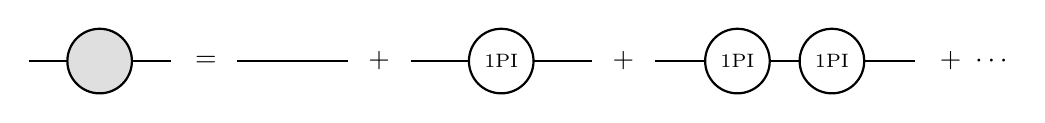
\begin{tikzpicture}[thick, baseline=(current bounding box.center),
        onepi/.style={draw, circle, fill=white, minimum size=0.82cm,
                      inner sep=0pt, font=\scriptsize},
        dressed/.style={draw, circle, fill=gray!25, minimum size=0.82cm,
                        inner sep=0pt}]
        \draw (0,0) -- (1.8,0);
        \node[dressed] at (0.9,0) {};
        \node at (2.25,0) {$=$};
        \draw (2.65,0) -- (4.05,0);
        \node at (4.45,0) {$+$};
        \draw (4.85,0) -- (7.15,0);
        \node[onepi] at (6.0,0) {1PI};
        \node at (7.55,0) {$+$};
        \draw (7.95,0) -- (11.25,0);
        \node[onepi] at (9.0,0) {1PI};
        \node[onepi] at (10.2,0) {1PI};
        \node at (12,0) {$+\ \cdots$};
    \end{tikzpicture}
    \end{center}
    \begin{solution}
        Note that at tree-level $\Gamma = S$, and therefore we can write
        \begin{equation}
            \Gamma_2(x,y) = G_0(x,y)^{-1} + \cdots, \quad \Gamma_2(x,y) \equiv \frac{\delta \Gamma[\varphi]}{\delta \varphi(x) \delta\varphi(y)}.
        \end{equation}
        In momentum space, this can be written as
        \begin{equation}
            \Gamma_2(k) = G_0(k)^{-1} +M^2(k) = \tilde{G}(k)^{-1},
        \end{equation}
        where $M^2(k)$ is the 1PI self-energy insertion.
        Using
        \begin{equation}
            \int d^dz\, \Gamma_2(x,z)G_\mathrm{CC}(z,y) = \delta^d (x-y), \quad \Gamma_2(x,y) \equiv \frac{\delta \Gamma[\varphi]}{\delta \varphi(x) \delta\varphi(y)}.
        \end{equation}
        This gives
        \begin{equation}
        \begin{aligned}
            \tilde{G}(k) &= \frac{1}{k^2 + m^2 +M^2(k)}\\
            &=\frac{1}{k^2+m^2}\sum_{n=0}^\infty\left(\frac{M^2(k)}{k^2+m^2}\right)^n,
        \end{aligned}
        \end{equation}
        which is exactly the geometric series.
    \end{solution}
\end{enumerate}
